\chapter{Scale setting}\addcontentsline{toc}{chapter}{Scale setting}

%%%%%%%%%%%%%%%%%%%%%%%%%%%%%%%%%%%%%%%%%%%%%%%%%%%%%%%%%%%
%%%%%%%%%%%%%%%%%%%%%%%%%%%%%%%%%%%%%%%%%%%%%%%%%%%%%%%%%%%
%%%%%%%%%%%%%%%%%%%%%%%%%%%%%%%%%%%%%%%%%%%%%%%%%%%%%%%%%%%
%%%%%%%%%%%%%%%%%%%%%%%%%%%%%%%%%%%%%%%%%%%%%%%%%%%%%%%%%%%

\label{ch_ss}

%%%%%%%%%%%%%%%%%%%%%%%%%%%%%%%%%%%%%%%%%%%%%%%%%%%%%%%%%%%
%%%%%%%%%%%%%%%%%%%%%%%%%%%%%%%%%%%%%%%%%%%%%%%%%%%%%%%%%%%
%%%%%%%%%%%%%%%%%%%%%%%%%%%%%%%%%%%%%%%%%%%%%%%%%%%%%%%%%%%
%%%%%%%%%%%%%%%%%%%%%%%%%%%%%%%%%%%%%%%%%%%%%%%%%%%%%%%%%%%

\section{Motivation}
\label{ch_ss:sec:introduction}

The scale setting involves the precise determination of one reference observable, the scale, in physical units, to which any other observable is compared in order to extract the value of the latter in physical units. 

We decide to use the gradient flow scale $t_0$ introduced in Sec.~\ref{ch_observables:sec:Flow} as an intermediate reference scale since it can be computed in the lattice with high precision. Following the discussion in Sec.~\ref{ch_foundation:sec:ss}, we choose for the phenomenological input the decay constants of the pion and kaon
\begin{equation}
\label{ch_ss:eq:fpik}
\Lambda\equiv f_{\pi K}=\frac{2}{3}\left(f_K+\frac{1}{2}f_{\pi}\right).
\end{equation}
After measuring $\sqrt{t_0}f_{\pi K}$ for each ensemble, one must perform a chiral-continuum limit in order to extract its value at the physical point and in the continuum. To define the physical point we use the pion and kaon masses, or equivalently the dimensionless quantities $\phi_2$ and $\phi_4$. For the determination of the physical value of these quantities we need again the physical value of $t_0$, which is the target of the analysis. As in Sec.~\ref{ch_ma}, we start with an initial guess in eq.~(\ref{ch_ma:eq:t0ph}) and iterate the analysis until convergence is observed. Since all lattice observables and the action that we use are $\mathcal{O}(a)$ improved, we expect lattice artifacts to start at $\mathcal{O}(a^2)$. In order to perform the chiral-continuum limit, we explore different ways of parameterizing the dependence on $\phi_2,\;\phi_4$ and on the lattice spacing $a$, and employ the same techniques of model averaging discussed in Sec.~\ref{ch_observables:sec:MA}.

After performing the chiral-continuum limit, using as external physical input the values of the pion and kaon decay constants we can determine the value of the scale $t_0$ as
\begin{equation}
\sqrt{t_0^{\textrm{ph}}}=\frac{\left.\begin{matrix}
\left(\sqrt{t_0}f_{\pi K}\right)^{\textrm{latt}}
\end{matrix}\right|_{a=0}}{f_{\pi K}^{\textrm{exp}}}.
\end{equation}

In particular, we are studying ensembles which employ $N_f=2+1$ fermions, and thus assume isospin symmetry for the light flavor. This means that the physical input for the masses and decay constants we need is not that of Nature, but that of isosymmetric QCD (isoQCD). These values are given by the Flavor Lattice Average Group (FLAG) in~\cite{FLAG21}
\begin{gather}
\label{ch_ss:eq:isoQCD}
m_{\pi}^{\textrm{isoQCD}}=134.9768(5)\;{\textrm{MeV}}, \quad
m_{K}^{\textrm{isoQCD}}=497.611(13)\;{\textrm{MeV}}, \\
f_{\pi}^{\textrm{isoQCD}}=130.56(2)_{\textrm{exp}}(13)_{\textrm{QED}}(2)_{|V_{ud}|}\;{\textrm{MeV}}, \quad \\
f_{K}^{\textrm{isoQCD}}=157.2(2)_{\textrm{exp}}(2)_{\textrm{QED}}(4)_{|V_{us}|}\;{\textrm{MeV}}.
\end{gather} 
As we see, the kaon decay constant receives a large contribution to its uncertainty from the determination of the $|V_{us}|$ CKM matrix element. Also, QED corrections are stronger in the kaon than in the pion. All these subtleties motivate a scale setting that uses only the pion decay constant as physical input. For this reason we also study this possibility when doing the model variation for the chiral-continuum extrapolation.

%%%%%%%%%%%%%%%%%%%%%%%%%%%%%%%%%%%%%%%%%%%%%%%%%%%%%%%%%%%
%%%%%%%%%%%%%%%%%%%%%%%%%%%%%%%%%%%%%%%%%%%%%%%%%%%%%%%%%%%
%%%%%%%%%%%%%%%%%%%%%%%%%%%%%%%%%%%%%%%%%%%%%%%%%%%%%%%%%%%
%%%%%%%%%%%%%%%%%%%%%%%%%%%%%%%%%%%%%%%%%%%%%%%%%%%%%%%%%%%


\section{Results}
\label{ch_ss:sec:Results}

The choice of the decay constants to set the scale, and in particular of the combination in eq.~(\ref{ch_ss:eq:fpik}) is due to its chiral behavior, since at fixed value of $\phi_4$ (as in our case thanks to the mass shifting procedure, see Sec.~\ref{ch_ma:sec:chiral_traj}) to NLO SU(3) ChPT it only depends on $\phi_2$ through chiral logarithms, 
\begin{align}
\label{ch_ss:eq:SU3ChPT}
&F_{\chi,\pi K}^{\textrm{cont}}(\phi_2)\equiv\left(\sqrt{8t_0}f_{\pi K}\right)^{\textrm{cont}}=\\
&=\frac{A}{4\pi}\left[1+\frac{7}{6}L\left(\frac{\phi_2}{A^2}\right)-\frac{4}{3}L\left(\frac{\phi_4-\frac{1}{2}\phi_2}{A^2}\right)-\frac{1}{2}L\left(\frac{\frac{4}{3}\phi_4-\phi_2}{A^2}\right)+B\phi_4\right],
\end{align}
with the chiral logarithms given by
\begin{equation}
\label{ch_ss:eq:log}
L(x)=x{\textrm{log}}\left(x\right),
\end{equation}
and $A,B$ related to chiral low energy constants (LEC). We use this expression to perform the chiral-continuum extrapolation of $\sqrt{t_0}f_{\pi K}$. Another possibility for the physical point extrapolation is to use Taylor expansions in $\phi_2$ around the symmetric point. We can either go to second or fourth order in the Taylor expansion
\begin{equation}
F_{\textrm{Tay},\pi K}^{\textrm{cont}}(\phi_2)\equiv\sqrt{8t_0}f_{\pi K}^{\textrm{cont}}=A+B\left(\phi_2-\phi_2^{\textrm{sym}}\right)^2,
\end{equation}
or
\begin{equation}
F_{\textrm{Tay},\pi K}^{\textrm{cont}}(\phi_2)=A+B\left(\phi_2-\phi_2^{\textrm{sym}}\right)^2+C\left(\phi_2-\phi_2^{\textrm{sym}}\right)^4.
\end{equation}
Due to symmetry reasons, there are no terms with odd powers of $\phi_2$~\cite{}.

Since the kaon decay constant is expected to receive more severe QED corrections than the pion, and the determination of its physical value for isosymmetric-QCD is affected by the uncertainty of the element of the CKM matrix $|V_{us}|$, we can also use the quantity $\sqrt{t_0}f_{\pi}$ to set the scale, and SU(2) ChPT to perform the physical point extrapolation. According to the latter,
\begin{align}
F_{\chi,\pi}^{\textrm{cont}}(\phi_2)\equiv\sqrt{8t_0}f_{\pi}^{\textrm{cont}}&=A\phi_2+B\left(1-2L\left(\frac{\phi_2}{B^2}\right)\right),\\
F_{\chi,K}^{\textrm{cont}}(\phi_2)\equiv\sqrt{8t_0}f_K^{\textrm{cont}}&=C\phi_2+D\left(1-\frac{3}{4}L\left(\frac{\phi_2}{B^2}\right)\right),
\end{align}
in which case we fit both $f_{\pi}$ and $f_K$ since they share a fit parameter, in order to help control the extrapolation in $f_{\pi}$. In the end, however, we set the scale only with external input for $f_{\pi}$.

In addition to the extrapolation in the pion mass, we need to supplement these fit functions with cutoff effects in order to describe our lattice data. For this we will explore two possibilities
\begin{align}
F^{\textrm{latt}}(\phi_2)&=F^{\textrm{cont}}(\phi_2)+W\frac{a^2}{8t_0},\\
F^{\textrm{latt}}(\phi_2)&=F^{\textrm{cont}}(\phi_2)+\left(W+Z\phi_2\right)\frac{a^2}{8t_0}.
\end{align}

In order to assess the systematic uncertainty in the extraction of $\sqrt{t_0}$, we will explore all these continuum-chiral extrapolations and their different results. In the same direction we also explore the impact of performing data cuts from the fits. In particular, we consider the following cuts (in addition to the ``no cut'' choice)
\begin{gather}
\beta>3.40, \quad
\beta>3.46, \quad
\phi_2<0.6, \\
\phi_2<0.4, \quad
\beta>3.40\;\&\;\phi_2<0.6, \\
m_{\pi}L>3.9, \quad
m_{\pi}L>4.0, \quad
m_{\pi}L>4.1.
\end{gather}

Finally, to perform all of these fits, we have two data sets: the Wilson unitary setup and the mixed action. Both must share the same continuum limit, but different cutoff effects. We can thus perform the continuum-chiral extrapolations for the Wilson data, for the mixed action, or for a combined data set, parameterizing the data with the same continuum limit behavior $F^{\textrm{cont}}(\phi_2)$ but different cutoff effects (different $W,Z$ fit parameters for Wilson and mixed action data). This third choice allows to further constrain the continuum extrapolation and keep it well under control, while increasing the statistics and getting better precision for $\sqrt{t_0}$. As a universality check, we perform the continuum limit of only symmetric point ensembles of both the Wilson and mixed action data, without imposing a common value in the continuum. Since all these points have the same $\phi_2$ they follow a line of constant physics as we approach the continuum. This extrapolation is shown in Fig.~\ref{ch_ss:fig:universality} and indeed it shows that both data sets agree perfectly well in the continuum, with the mixed action data having much milder cutoff effects.

Once the various models to extrapolate to the continuum and physical point have been explored, we use the model averaging technique in Sec.~\ref{ch_observables:sec:MA} to assign a weight to each model 
\begin{equation}
W\propto\exp\left(-\frac{1}{2}\left(\chi^2-2\left<\chi^2\right>\right)\right),
\end{equation}
that allows us to compute a weighted average for $\sqrt{t_0}$, as well as the associated systematic uncertainty
\begin{align}
\left<\sqrt{t_0}\right>&=\sum_i\sqrt{t_0^{(i)}}W^{(i)},\\
\sigma^2_{\textrm{syst}}&=\left<\sqrt{t_0}^2\right>-\left<\sqrt{t_0}\right>^2.
\end{align}

In Figs.~\ref{ch_ss:fig:model_av} we show the model average results for the Wilson unitary setup, for the mixed action and for the combined analysis. In Table~\ref{ch_ss:tab:t0_models} we show the numerical results of $\sqrt{t_0}$ for each model considered, together with their weights and p-values. In Fig.~\ref{ch_ss:fig:SU3} we show the continuum-chiral extrapolation for one of the best models explored in terms of the TIC for the mixed action, Wilson and combined data sets.

The final results for $\sqrt{t_0}$ in physical units as computed from the model average for the different data sets are
\begin{align}
\sqrt{t_0}&=0.1434(7)_{\textrm{stat}}(3)_{\textrm{syst}}\;\textrm{fm, Wilson}, \\
\sqrt{t_0}&=0.1435(8)_{\textrm{stat}}(7)_{\textrm{syst}}\;\textrm{fm, Mixed action}, \\
\sqrt{t_0}&=0.1437(6)_{\textrm{stat}}(4)_{\textrm{syst}}\;\textrm{fm, Combined}.
\end{align}

\begin{figure}
    \centering
    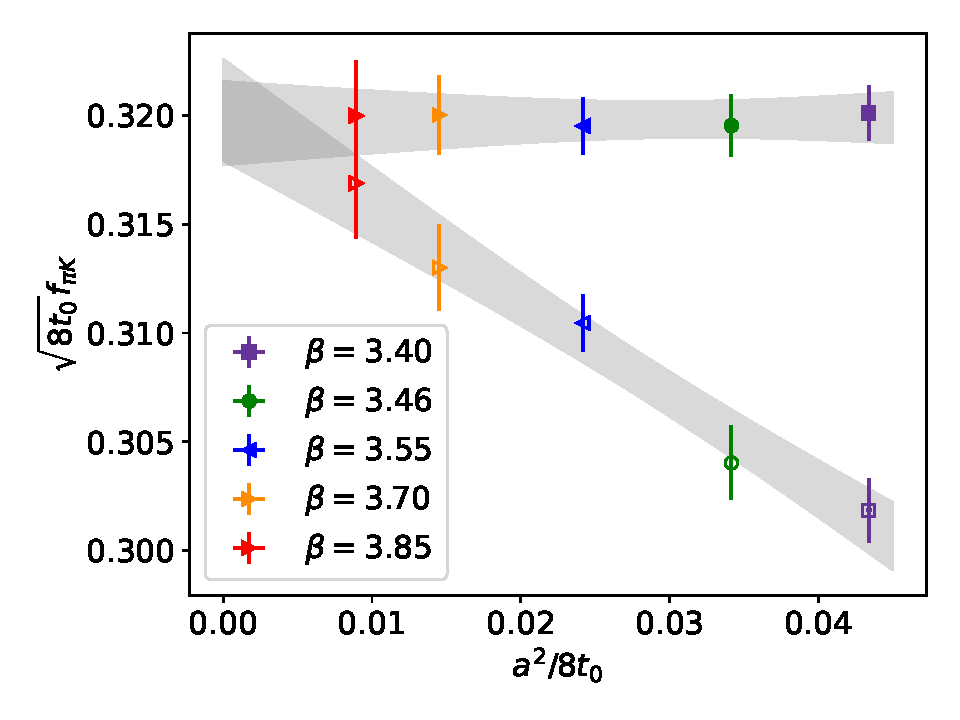
\includegraphics[width=1.\textwidth]{./cap5/figs/continuum_sym.pdf}
    \caption{Continuum limit of symmetric point ensembles for the Wilson unitary results or sea data set (empty points) and for the mixed action results (filled points). A common continuum limit is not imposed. Cutoff effects are parameterized as pure $\mathcal{O}(a^2)$ artifacts.}
    \label{ch_ss:fig:universality}
\end{figure}

\begin{figure}
    \centering
    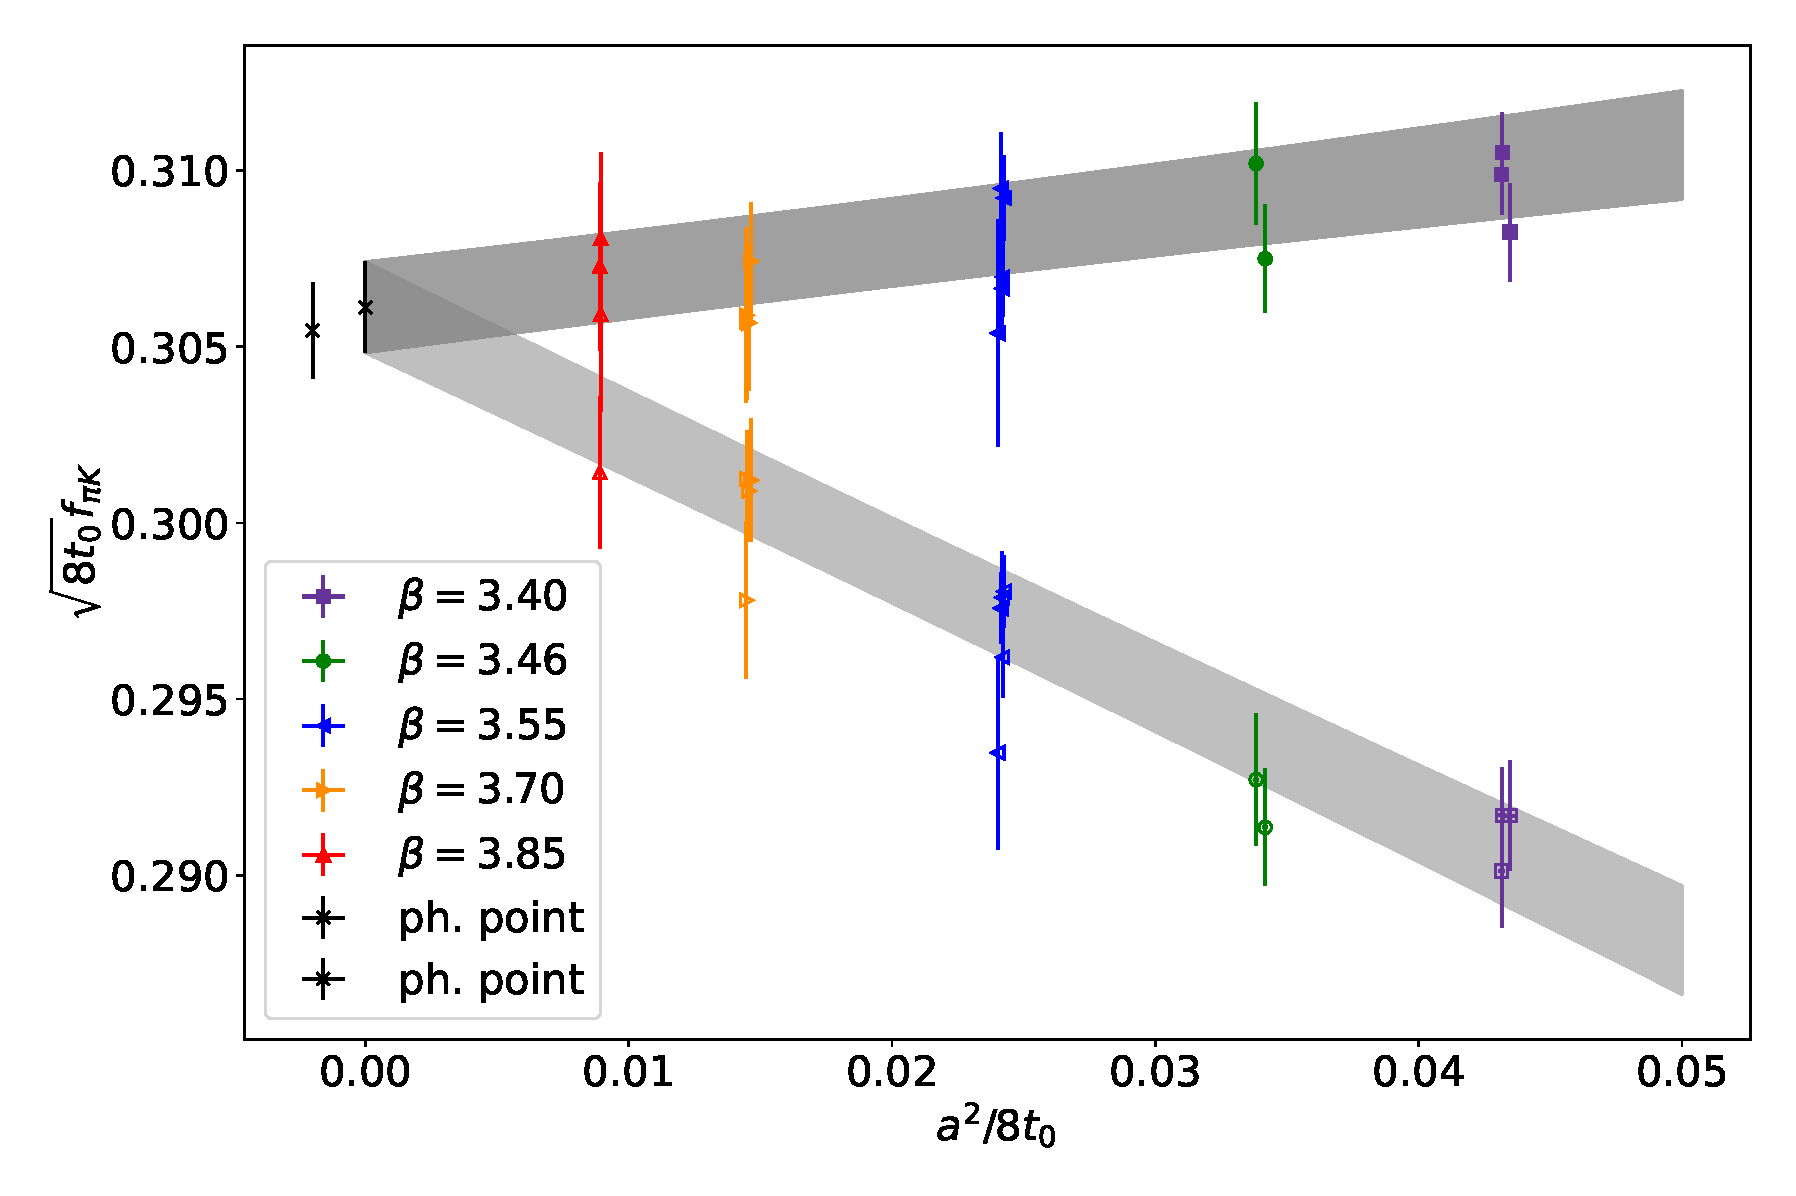
\includegraphics[width=1.\textwidth]{./cap5/figs/SU3a2_projection.pdf}
    \caption{}
    \label{ch_ss:fig:}
\end{figure}

\begin{figure}
    \centering
    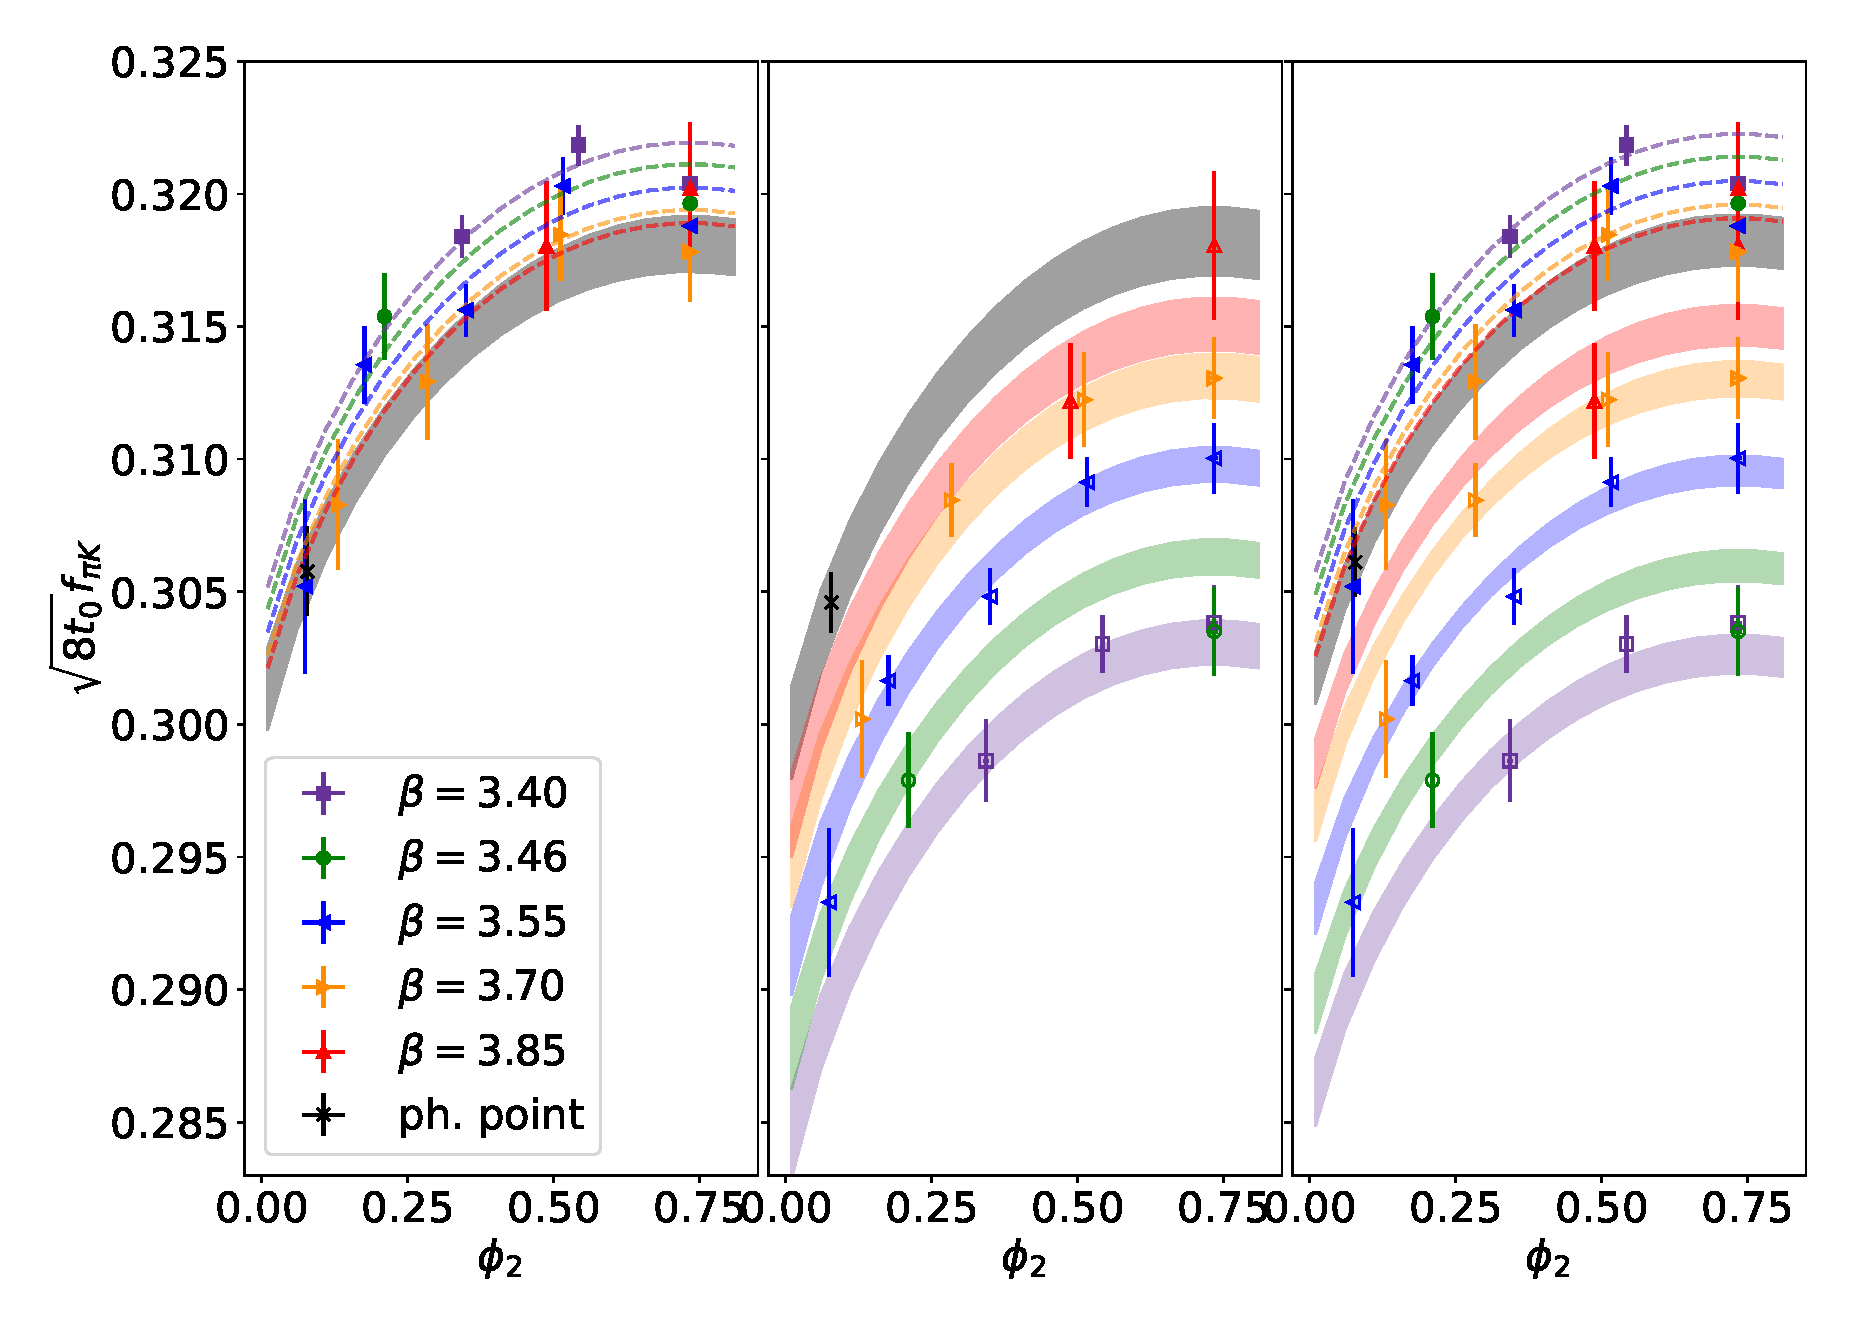
\includegraphics[width=1.\textwidth]{./cap5/figs/SU3.pdf}
    \caption{}
    \label{ch_ss:fig:}
\end{figure}

\begin{figure}
    \centering
    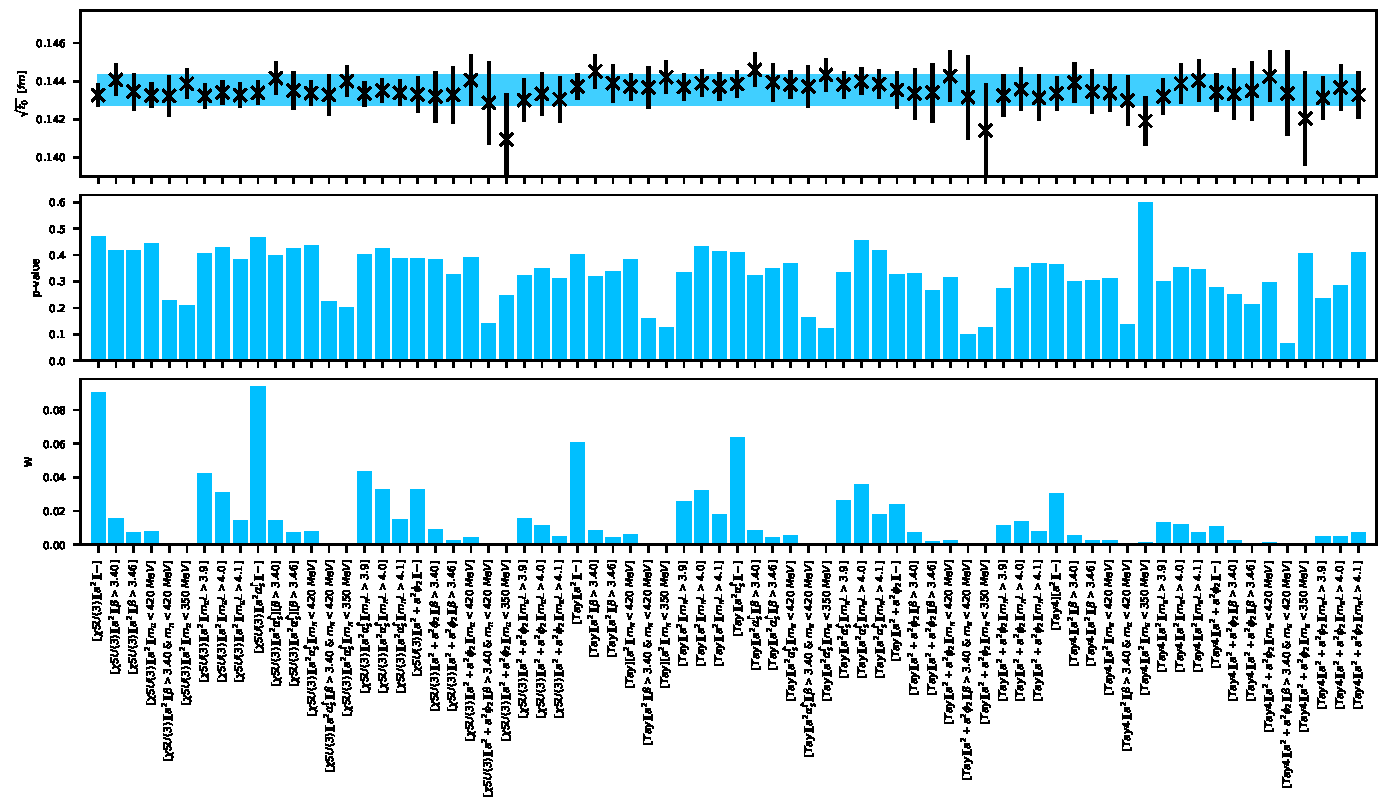
\includegraphics[width=1.\textwidth]{./cap5/figs/BMA_w.pdf}
    \caption{}
    \label{ch_ss:fig:}
\end{figure}

\begin{figure}
    \centering
    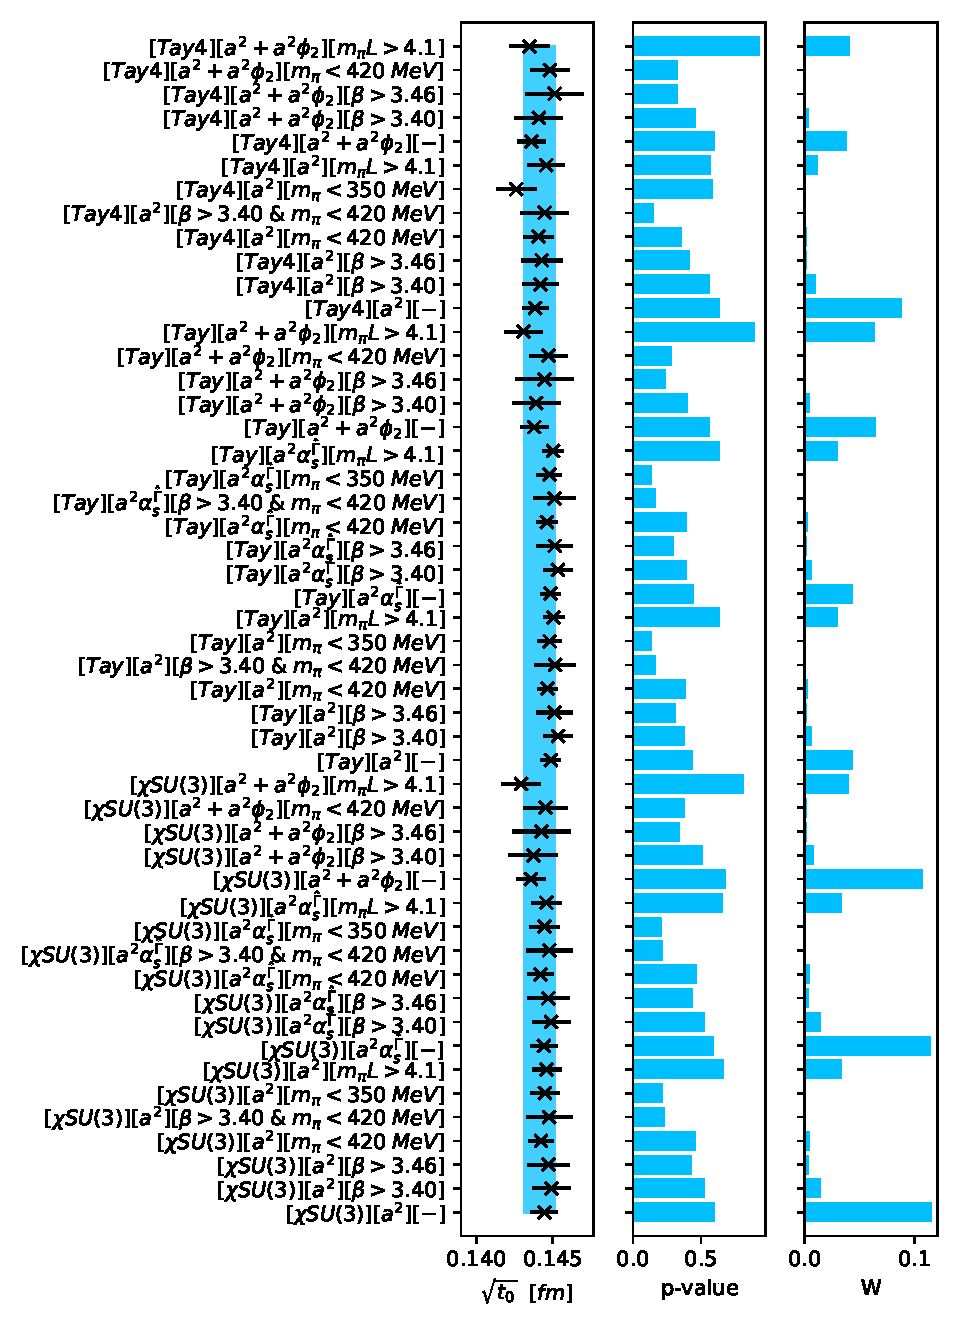
\includegraphics[width=1.\textwidth]{./cap5/figs/BMA_tm.pdf}
    \caption{}
    \label{ch_ss:fig:}
\end{figure}

\begin{figure}
    \centering
    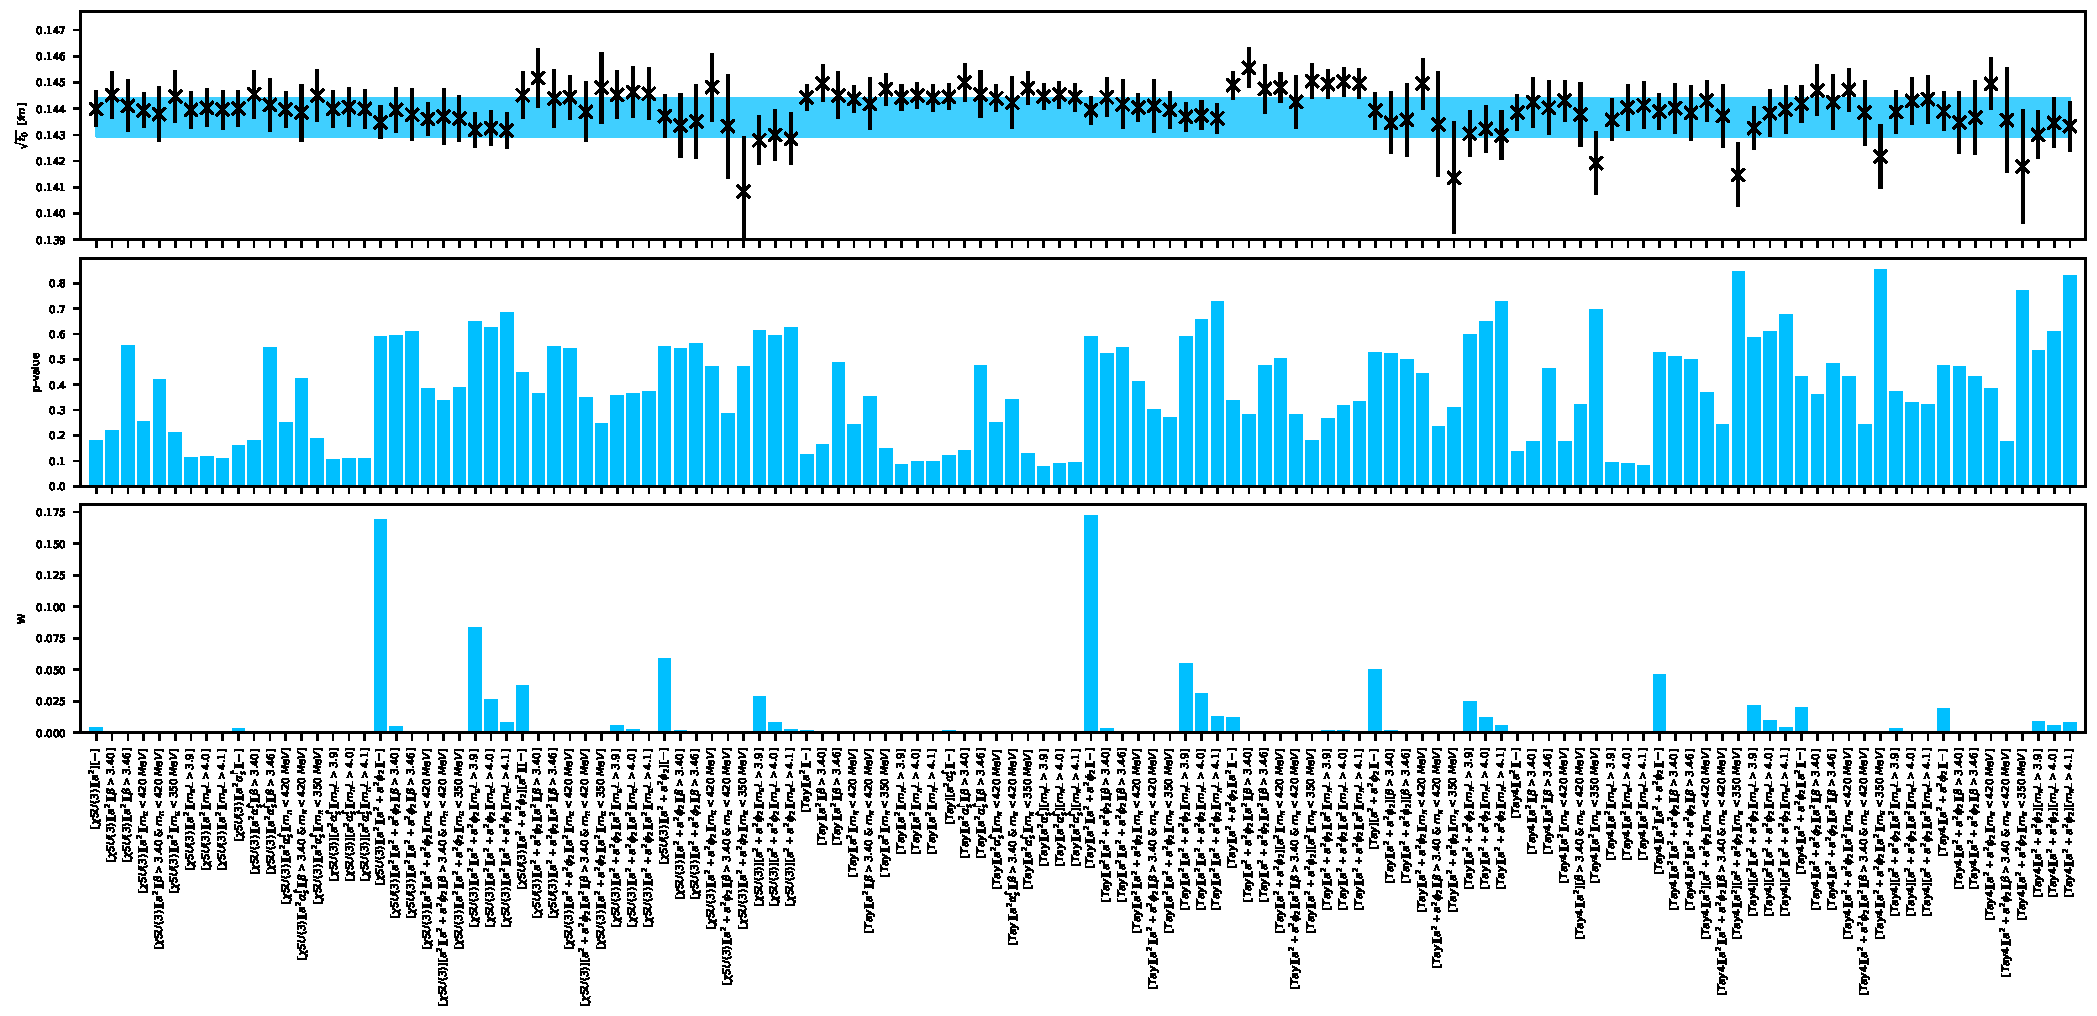
\includegraphics[width=1.\textwidth]{./cap5/figs/BMA_comb.pdf}
    \caption{}
    \label{ch_ss:fig:}
\end{figure}

\begin{longtable}{ c | c | c | c }
\toprule
 & p-value & $W$ & $\sqrt{t_0}$ [fm] \\
\midrule
$[\chi SU(3)][a^2][-]$ & 0.4742 & 0.0901 & 0.1433(6) \\
$[\chi SU(3)][a^2][\beta>3.40]$ & 0.4036 & 0.0153 & 0.1441(8) \\
$[\chi SU(3)][a^2][\beta>3.46]$ & 0.4376 & 0.0071 & 0.1434(10) \\
$[\chi SU(3)][a^2][m_{\pi}<420\;MeV]$ & 0.4424 & 0.0079 & 0.1433(7) \\
$[\chi SU(3)][a^2][\beta>3.40\;\&\;m_{\pi}<420\;MeV]$ & 0.2264 & 0.0007 & 0.1432(11) \\
$[\chi SU(3)][a^2][m_{\pi}<350\;MeV]$ & 0.1998 & 0.0004 & 0.1439(8) \\
$[\chi SU(3)][a^2][m_{\pi}L>3.9]$ & 0.4072 & 0.0421 & 0.1432(6) \\
$[\chi SU(3)][a^2][m_{\pi}L>4.0]$ & 0.4402 & 0.0312 & 0.1434(6) \\
$[\chi SU(3)][a^2][m_{\pi}L>4.1]$ & 0.3846 & 0.0145 & 0.1433(7) \\
$[\chi SU(3)][a^2\alpha_s^{\hat{\Gamma}}][-]$ & 0.4688 & 0.0936 & 0.1434(6) \\
$[\chi SU(3)][a^2\alpha_s^{\hat{\Gamma}}][\beta>3.40]$ & 0.4012 & 0.0145 & 0.1442(9) \\
$[\chi SU(3)][a^2\alpha_s^{\hat{\Gamma}}][\beta>3.46]$ & 0.4386 & 0.0071 & 0.1435(10) \\
$[\chi SU(3)][a^2\alpha_s^{\hat{\Gamma}}][m_{\pi}<420\;MeV]$ & 0.4398 & 0.008 & 0.1434(7) \\
$[\chi SU(3)][a^2\alpha_s^{\hat{\Gamma}}][\beta>3.40\;\&\;m_{\pi}<420\;MeV]$ & 0.2254 & 0.0007 & 0.1433(11) \\
$[\chi SU(3)][a^2\alpha_s^{\hat{\Gamma}}][m_{\pi}<350\;MeV]$ & 0.2112 & 0.0004 & 0.144(8) \\
$[\chi SU(3)][a^2\alpha_s^{\hat{\Gamma}}][m_{\pi}L>3.9]$ & 0.4008 & 0.0434 & 0.1433(6) \\
$[\chi SU(3)][a^2\alpha_s^{\hat{\Gamma}}][m_{\pi}L>4.0]$ & 0.4368 & 0.0326 & 0.1435(6) \\
$[\chi SU(3)][a^2\alpha_s^{\hat{\Gamma}}][m_{\pi}L>4.1]$ & 0.3788 & 0.0147 & 0.1434(7) \\
$[\chi SU(3)][a^2+a^2\phi_2][-]$ & 0.389 & 0.0329 & 0.1433(10) \\
$[\chi SU(3)][a^2+a^2\phi_2][\beta>3.40]$ & 0.3814 & 0.0093 & 0.1432(13) \\
$[\chi SU(3)][a^2+a^2\phi_2][\beta>3.46]$ & 0.3268 & 0.0028 & 0.1433(15) \\
$[\chi SU(3)][a^2+a^2\phi_2][m_{\pi}<420\;MeV]$ & 0.3814 & 0.0041 & 0.1441(13) \\
$[\chi SU(3)][a^2+a^2\phi_2][\beta>3.40\;\&\;m_{\pi}<420\;MeV]$ & 0.1362 & 0.0003 & 0.1429(22) \\
$[\chi SU(3)][a^2+a^2\phi_2][m_{\pi}<350\;MeV]$ & 0.241 & 0.0003 & 0.1409(24) \\
$[\chi SU(3)][a^2+a^2\phi_2][m_{\pi}L>3.9]$ & 0.3324 & 0.0156 & 0.143(11) \\
$[\chi SU(3)][a^2+a^2\phi_2][m_{\pi}L>4.0]$ & 0.3418 & 0.0112 & 0.1433(11) \\
$[\chi SU(3)][a^2+a^2\phi_2][m_{\pi}L>4.1]$ & 0.3048 & 0.0049 & 0.1431(12) \\
$[Tay][a^2][-]$ & 0.409 & 0.0607 & 0.1437(7) \\
$[Tay][a^2][\beta>3.40]$ & 0.3242 & 0.0084 & 0.1445(9) \\
$[Tay][a^2][\beta>3.46]$ & 0.3536 & 0.0044 & 0.1439(10) \\
$[Tay][a^2][m_{\pi}<420\;MeV]$ & 0.3784 & 0.0058 & 0.1437(7) \\
$[Tay][a^2][\beta>3.40\;\&\;m_{\pi}<420\;MeV]$ & 0.1646 & 0.0004 & 0.1437(11) \\
$[Tay][a^2][m_{\pi}<350\;MeV]$ & 0.1284 & 0.0002 & 0.1442(9) \\
$[Tay][a^2][m_{\pi}L>3.9]$ & 0.3364 & 0.0259 & 0.1437(7) \\
$[Tay][a^2][m_{\pi}L>4.0]$ & 0.4432 & 0.0322 & 0.1439(7) \\
$[Tay][a^2][m_{\pi}L>4.1]$ & 0.4212 & 0.0181 & 0.1437(7) \\
$[Tay][a^2\alpha_s^{\hat{\Gamma}}][-]$ & 0.403 & 0.0638 & 0.1439(7) \\
$[Tay][a^2\alpha_s^{\hat{\Gamma}}][\beta>3.40]$ & 0.3114 & 0.0087 & 0.1446(9) \\
$[Tay][a^2\alpha_s^{\hat{\Gamma}}][\beta>3.46]$ & 0.3538 & 0.0045 & 0.144(10) \\
$[Tay][a^2\alpha_s^{\hat{\Gamma}}][m_{\pi}<420\;MeV]$ & 0.3718 & 0.0057 & 0.1438(7) \\
$[Tay][a^2\alpha_s^{\hat{\Gamma}}][\beta>3.40\;\&\;m_{\pi}<420\;MeV]$ & 0.1628 & 0.0004 & 0.1437(11) \\
$[Tay][a^2\alpha_s^{\hat{\Gamma}}][m_{\pi}<350\;MeV]$ & 0.1248 & 0.0002 & 0.1443(9) \\
$[Tay][a^2\alpha_s^{\hat{\Gamma}}][m_{\pi}L>3.9]$ & 0.3398 & 0.0265 & 0.1438(7) \\
$[Tay][a^2\alpha_s^{\hat{\Gamma}}][m_{\pi}L>4.0]$ & 0.4418 & 0.036 & 0.144(7) \\
$[Tay][a^2\alpha_s^{\hat{\Gamma}}][m_{\pi}L>4.1]$ & 0.4308 & 0.0181 & 0.1438(7) \\
$[Tay][a^2+a^2\phi_2][-]$ & 0.3188 & 0.0237 & 0.1435(10) \\
$[Tay][a^2+a^2\phi_2][\beta>3.40]$ & 0.3406 & 0.0071 & 0.1433(13) \\
$[Tay][a^2+a^2\phi_2][\beta>3.46]$ & 0.2508 & 0.0019 & 0.1434(15) \\
$[Tay][a^2+a^2\phi_2][m_{\pi}<420\;MeV]$ & 0.3182 & 0.0023 & 0.1443(13) \\
$[Tay][a^2+a^2\phi_2][\beta>3.40\;\&\;m_{\pi}<420\;MeV]$ & 0.0988 & 0.0002 & 0.1431(22) \\
$[Tay][a^2+a^2\phi_2][m_{\pi}<350\;MeV]$ & 0.1232 & 0.0002 & 0.1414(25) \\
$[Tay][a^2+a^2\phi_2][m_{\pi}L>3.9]$ & 0.2772 & 0.0116 & 0.1433(11) \\
$[Tay][a^2+a^2\phi_2][m_{\pi}L>4.0]$ & 0.3542 & 0.0136 & 0.1436(11) \\
$[Tay][a^2+a^2\phi_2][m_{\pi}L>4.1]$ & 0.3706 & 0.0076 & 0.1431(12) \\
$[Tay4][a^2][-]$ & 0.3524 & 0.0302 & 0.1434(9) \\
$[Tay4][a^2][\beta>3.40]$ & 0.3096 & 0.0052 & 0.1439(11) \\
$[Tay4][a^2][\beta>3.46]$ & 0.3022 & 0.0022 & 0.1435(11) \\
$[Tay4][a^2][m_{\pi}<420\;MeV]$ & 0.3256 & 0.0022 & 0.1434(10) \\
$[Tay4][a^2][\beta>3.40\;\&\;m_{\pi}<420\;MeV]$ & 0.131 & 0.0002 & 0.143(13) \\
$[Tay4][a^2][m_{\pi}<350\;MeV]$ & 0.6076 & 0.0011 & 0.1419(13) \\
$[Tay4][a^2][m_{\pi}L>3.9]$ & 0.3106 & 0.0131 & 0.1432(9) \\
$[Tay4][a^2][m_{\pi}L>4.0]$ & 0.3498 & 0.0121 & 0.1439(11) \\
$[Tay4][a^2][m_{\pi}L>4.1]$ & 0.3464 & 0.007 & 0.144(11) \\
$[Tay4][a^2+a^2\phi_2][-]$ & 0.2874 & 0.0105 & 0.1434(10) \\
$[Tay4][a^2+a^2\phi_2][\beta>3.40]$ & 0.273 & 0.0027 & 0.1433(13) \\
$[Tay4][a^2+a^2\phi_2][\beta>3.46]$ & 0.217 & 0.0009 & 0.1435(15) \\
$[Tay4][a^2+a^2\phi_2][m_{\pi}<420\;MeV]$ & 0.2864 & 0.0014 & 0.1443(13) \\
$[Tay4][a^2+a^2\phi_2][\beta>3.40\;\&\;m_{\pi}<420\;MeV]$ & 0.0736 & 0.0001 & 0.1434(22) \\
$[Tay4][a^2+a^2\phi_2][m_{\pi}<350\;MeV]$ & 0.4098 & 0.0004 & 0.142(25) \\
$[Tay4][a^2+a^2\phi_2][m_{\pi}L>3.9]$ & 0.2404 & 0.0049 & 0.1431(11) \\
$[Tay4][a^2+a^2\phi_2][m_{\pi}L>4.0]$ & 0.2872 & 0.0049 & 0.1437(12) \\
$[Tay4][a^2+a^2\phi_2][m_{\pi}L>4.1]$ & 0.4026 & 0.007 & 0.1433(12) \\
\bottomrule
\caption{Wilson}
\end{longtable}

\begin{longtable}{ c | c | c | c }
\toprule
 & p-value & $W$ & $\sqrt{t_0}$ [fm] \\
\midrule
$[\chi SU(3)][a^2][-]$ & 0.809 & 0.0825 & 0.1438(8) \\
$[\chi SU(3)][a^2][\beta>3.40]$ & 0.7188 & 0.0075 & 0.1441(11) \\
$[\chi SU(3)][a^2][\beta>3.46]$ & 0.7836 & 0.0031 & 0.1441(12) \\
$[\chi SU(3)][a^2][m_{\pi}<420\;MeV]$ & 0.7636 & 0.0029 & 0.1438(8) \\
$[\chi SU(3)][a^2][\beta>3.40\;\&\;m_{\pi}<420\;MeV]$ & 0.6494 & 0.0003 & 0.1438(13) \\
$[\chi SU(3)][a^2][m_{\pi}<350\;MeV]$ & 0.5908 & 0.0002 & 0.1439(13) \\
$[\chi SU(3)][a^2][m_{\pi}L>3.9]$ & 0.7484 & 0.0303 & 0.1438(8) \\
$[\chi SU(3)][a^2][m_{\pi}L>4.0]$ & 0.7176 & 0.0136 & 0.1439(9) \\
$[\chi SU(3)][a^2][m_{\pi}L>4.1]$ & 0.635 & 0.0059 & 0.144(9) \\
$[\chi SU(3)][a^2\alpha_s^{\hat{\Gamma}}][-]$ & 0.8192 & 0.0819 & 0.1438(8) \\
$[\chi SU(3)][a^2\alpha_s^{\hat{\Gamma}}][\beta>3.40]$ & 0.7294 & 0.0074 & 0.1441(11) \\
$[\chi SU(3)][a^2\alpha_s^{\hat{\Gamma}}][\beta>3.46]$ & 0.7774 & 0.0031 & 0.1441(12) \\
$[\chi SU(3)][a^2\alpha_s^{\hat{\Gamma}}][m_{\pi}<420\;MeV]$ & 0.7498 & 0.0028 & 0.1437(8) \\
$[\chi SU(3)][a^2\alpha_s^{\hat{\Gamma}}][\beta>3.40\;\&\;m_{\pi}<420\;MeV]$ & 0.642 & 0.0003 & 0.1438(13) \\
$[\chi SU(3)][a^2\alpha_s^{\hat{\Gamma}}][m_{\pi}<350\;MeV]$ & 0.5908 & 0.0002 & 0.1438(13) \\
$[\chi SU(3)][a^2\alpha_s^{\hat{\Gamma}}][m_{\pi}L>3.9]$ & 0.7486 & 0.0298 & 0.1438(9) \\
$[\chi SU(3)][a^2\alpha_s^{\hat{\Gamma}}][m_{\pi}L>4.0]$ & 0.7046 & 0.0135 & 0.1439(9) \\
$[\chi SU(3)][a^2\alpha_s^{\hat{\Gamma}}][m_{\pi}L>4.1]$ & 0.6452 & 0.0058 & 0.144(9) \\
$[\chi SU(3)][a^2+a^2\phi_2][-]$ & 0.868 & 0.0678 & 0.143(10) \\
$[\chi SU(3)][a^2+a^2\phi_2][\beta>3.40]$ & 0.849 & 0.0081 & 0.1423(16) \\
$[\chi SU(3)][a^2+a^2\phi_2][\beta>3.46]$ & 0.7768 & 0.0016 & 0.1429(18) \\
$[\chi SU(3)][a^2+a^2\phi_2][m_{\pi}<420\;MeV]$ & 0.6692 & 0.0011 & 0.1438(14) \\
$[\chi SU(3)][a^2+a^2\phi_2][\beta>3.40\;\&\;m_{\pi}<420\;MeV]$ & 0.517 & 0.0001 & 0.1435(26) \\
$[\chi SU(3)][a^2+a^2\phi_2][m_{\pi}<350\;MeV]$ & 0.778 & 0.0001 & 0.1407(25) \\
$[\chi SU(3)][a^2+a^2\phi_2][m_{\pi}L>3.9]$ & 0.9316 & 0.0609 & 0.1422(11) \\
$[\chi SU(3)][a^2+a^2\phi_2][m_{\pi}L>4.0]$ & 0.8984 & 0.0246 & 0.1423(12) \\
$[\chi SU(3)][a^2+a^2\phi_2][m_{\pi}L>4.1]$ & 0.8536 & 0.0098 & 0.1424(12) \\
$[Tay][a^2][-]$ & 0.723 & 0.0486 & 0.1443(6) \\
$[Tay][a^2][\beta>3.40]$ & 0.625 & 0.0049 & 0.1445(9) \\
$[Tay][a^2][\beta>3.46]$ & 0.7244 & 0.0024 & 0.1445(11) \\
$[Tay][a^2][m_{\pi}<420\;MeV]$ & 0.7746 & 0.0029 & 0.1442(6) \\
$[Tay][a^2][\beta>3.40\;\&\;m_{\pi}<420\;MeV]$ & 0.6724 & 0.0003 & 0.1442(13) \\
$[Tay][a^2][m_{\pi}<350\;MeV]$ & 0.4904 & 0.0001 & 0.1441(8) \\
$[Tay][a^2][m_{\pi}L>3.9]$ & 0.6628 & 0.0177 & 0.1443(6) \\
$[Tay][a^2][m_{\pi}L>4.0]$ & 0.6514 & 0.0104 & 0.1444(6) \\
$[Tay][a^2][m_{\pi}L>4.1]$ & 0.575 & 0.0043 & 0.1445(7) \\
$[Tay][a^2\alpha_s^{\hat{\Gamma}}][-]$ & 0.7372 & 0.0475 & 0.1443(6) \\
$[Tay][a^2\alpha_s^{\hat{\Gamma}}][\beta>3.40]$ & 0.631 & 0.0049 & 0.1445(9) \\
$[Tay][a^2\alpha_s^{\hat{\Gamma}}][\beta>3.46]$ & 0.7248 & 0.0024 & 0.1445(11) \\
$[Tay][a^2\alpha_s^{\hat{\Gamma}}][m_{\pi}<420\;MeV]$ & 0.7628 & 0.003 & 0.1442(6) \\
$[Tay][a^2\alpha_s^{\hat{\Gamma}}][\beta>3.40\;\&\;m_{\pi}<420\;MeV]$ & 0.6448 & 0.0003 & 0.1442(13) \\
$[Tay][a^2\alpha_s^{\hat{\Gamma}}][m_{\pi}<350\;MeV]$ & 0.5006 & 0.0001 & 0.1441(8) \\
$[Tay][a^2\alpha_s^{\hat{\Gamma}}][m_{\pi}L>3.9]$ & 0.655 & 0.0175 & 0.1443(6) \\
$[Tay][a^2\alpha_s^{\hat{\Gamma}}][m_{\pi}L>4.0]$ & 0.6554 & 0.0104 & 0.1444(7) \\
$[Tay][a^2\alpha_s^{\hat{\Gamma}}][m_{\pi}L>4.1]$ & 0.5842 & 0.0043 & 0.1445(7) \\
$[Tay][a^2+a^2\phi_2][-]$ & 0.8866 & 0.0787 & 0.1432(9) \\
$[Tay][a^2+a^2\phi_2][\beta>3.40]$ & 0.869 & 0.0093 & 0.1422(16) \\
$[Tay][a^2+a^2\phi_2][\beta>3.46]$ & 0.7962 & 0.0018 & 0.1427(19) \\
$[Tay][a^2+a^2\phi_2][m_{\pi}<420\;MeV]$ & 0.6716 & 0.0012 & 0.1438(12) \\
$[Tay][a^2+a^2\phi_2][\beta>3.40\;\&\;m_{\pi}<420\;MeV]$ & 0.5496 & 0.0001 & 0.1431(28) \\
$[Tay][a^2+a^2\phi_2][m_{\pi}<350\;MeV]$ & 0.6412 & 0.0001 & 0.1408(26) \\
$[Tay][a^2+a^2\phi_2][m_{\pi}L>3.9]$ & 0.929 & 0.0676 & 0.1424(11) \\
$[Tay][a^2+a^2\phi_2][m_{\pi}L>4.0]$ & 0.9378 & 0.0343 & 0.1426(11) \\
$[Tay][a^2+a^2\phi_2][m_{\pi}L>4.1]$ & 0.893 & 0.0126 & 0.1426(11) \\
$[Tay4][a^2][-]$ & 0.7656 & 0.0341 & 0.1436(9) \\
$[Tay4][a^2][\beta>3.40]$ & 0.6486 & 0.0031 & 0.1437(12) \\
$[Tay4][a^2][\beta>3.46]$ & 0.694 & 0.0011 & 0.144(13) \\
$[Tay4][a^2][m_{\pi}<420\;MeV]$ & 0.6632 & 0.0011 & 0.1442(10) \\
$[Tay4][a^2][\beta>3.40\;\&\;m_{\pi}<420\;MeV]$ & 0.5278 & 0.0001 & 0.1442(15) \\
$[Tay4][a^2][m_{\pi}<350\;MeV]$ & 0.9038 & 0.0002 & 0.1422(14) \\
$[Tay4][a^2][m_{\pi}L>3.9]$ & 0.7218 & 0.0152 & 0.1433(10) \\
$[Tay4][a^2][m_{\pi}L>4.0]$ & 0.6704 & 0.0057 & 0.1435(12) \\
$[Tay4][a^2][m_{\pi}L>4.1]$ & 0.6172 & 0.0027 & 0.1435(12) \\
$[Tay4][a^2+a^2\phi_2][-]$ & 0.8398 & 0.0295 & 0.1433(9) \\
$[Tay4][a^2+a^2\phi_2][\beta>3.40]$ & 0.8008 & 0.0036 & 0.1422(16) \\
$[Tay4][a^2+a^2\phi_2][\beta>3.46]$ & 0.6998 & 0.0007 & 0.1426(20) \\
$[Tay4][a^2+a^2\phi_2][m_{\pi}<420\;MeV]$ & 0.5982 & 0.0005 & 0.1438(12) \\
$[Tay4][a^2+a^2\phi_2][\beta>3.40\;\&\;m_{\pi}<420\;MeV]$ & 0.391 & 0.0001 & 0.1428(28) \\
$[Tay4][a^2+a^2\phi_2][m_{\pi}<350\;MeV]$ & 0.7958 & 0.0001 & 0.1415(27) \\
$[Tay4][a^2+a^2\phi_2][m_{\pi}L>3.9]$ & 0.8956 & 0.0245 & 0.1425(11) \\
$[Tay4][a^2+a^2\phi_2][m_{\pi}L>4.0]$ & 0.9454 & 0.0182 & 0.1431(12) \\
$[Tay4][a^2+a^2\phi_2][m_{\pi}L>4.1]$ & 0.8974 & 0.0067 & 0.143(12) \\
\bottomrule
\caption{Wtm}
\end{longtable}

\begin{longtable}{ c | c | c | c }
\toprule
 & p-value & $W$ & $\sqrt{t_0}$ [fm] \\
\midrule
$[\chi SU(3)][a^2][-]$ & 0.1726 & 0.004 & 0.144(7) \\
$[\chi SU(3)][a^2][\beta>3.40]$ & 0.224 & 0.0004 & 0.1445(9) \\
$[\chi SU(3)][a^2][\beta>3.46]$ & 0.5646 & 0.0007 & 0.1441(10) \\
$[\chi SU(3)][a^2][m_{\pi}<420\;MeV]$ & 0.2606 & 0.0001 & 0.1439(7) \\
$[\chi SU(3)][a^2][\beta>3.40\;\&\;m_{\pi}<420\;MeV]$ & 0.4156 & 0.0 & 0.1438(11) \\
$[\chi SU(3)][a^2][m_{\pi}<350\;MeV]$ & 0.2024 & 0.0 & 0.1445(10) \\
$[\chi SU(3)][a^2][m_{\pi}L>3.9]$ & 0.1176 & 0.0004 & 0.144(7) \\
$[\chi SU(3)][a^2][m_{\pi}L>4.0]$ & 0.1116 & 0.0001 & 0.144(7) \\
$[\chi SU(3)][a^2][m_{\pi}L>4.1]$ & 0.11 & 0.0001 & 0.144(7) \\
$[\chi SU(3)][a^2\alpha_s^{\hat{\Gamma}}][-]$ & 0.164 & 0.0037 & 0.144(7) \\
$[\chi SU(3)][a^2\alpha_s^{\hat{\Gamma}}][\beta>3.40]$ & 0.1658 & 0.0002 & 0.1445(9) \\
$[\chi SU(3)][a^2\alpha_s^{\hat{\Gamma}}][\beta>3.46]$ & 0.5594 & 0.0007 & 0.1441(10) \\
$[\chi SU(3)][a^2\alpha_s^{\hat{\Gamma}}][m_{\pi}<420\;MeV]$ & 0.232 & 0.0001 & 0.144(7) \\
$[\chi SU(3)][a^2\alpha_s^{\hat{\Gamma}}][\beta>3.40\;\&\;m_{\pi}<420\;MeV]$ & 0.4224 & 0.0 & 0.1438(11) \\
$[\chi SU(3)][a^2\alpha_s^{\hat{\Gamma}}][m_{\pi}<350\;MeV]$ & 0.1994 & 0.0 & 0.1445(10) \\
$[\chi SU(3)][a^2\alpha_s^{\hat{\Gamma}}][m_{\pi}L>3.9]$ & 0.1048 & 0.0004 & 0.144(7) \\
$[\chi SU(3)][a^2\alpha_s^{\hat{\Gamma}}][m_{\pi}L>4.0]$ & 0.0932 & 0.0001 & 0.1441(7) \\
$[\chi SU(3)][a^2\alpha_s^{\hat{\Gamma}}][m_{\pi}L>4.1]$ & 0.0962 & 0.0 & 0.144(7) \\
$[\chi SU(3)][a^2][a^2+a^2\phi_2][-]$ & 0.5966 & 0.1694 & 0.1435(6) \\
$[\chi SU(3)][a^2][a^2+a^2\phi_2][\beta>3.40]$ & 0.588 & 0.0048 & 0.144(9) \\
$[\chi SU(3)][a^2][a^2+a^2\phi_2][\beta>3.46]$ & 0.6146 & 0.0006 & 0.1438(10) \\
$[\chi SU(3)][a^2][a^2+a^2\phi_2][m_{\pi}<420\;MeV]$ & 0.3844 & 0.0002 & 0.1436(6) \\
$[\chi SU(3)][a^2][a^2+a^2\phi_2][\beta>3.40\;\&\;m_{\pi}<420\;MeV]$ & 0.347 & 0.0 & 0.1437(11) \\
$[\chi SU(3)][a^2][a^2+a^2\phi_2][m_{\pi}<350\;MeV]$ & 0.3836 & 0.0 & 0.1436(9) \\
$[\chi SU(3)][a^2][a^2+a^2\phi_2][m_{\pi}L>3.9]$ & 0.6536 & 0.0836 & 0.1432(7) \\
$[\chi SU(3)][a^2][a^2+a^2\phi_2][m_{\pi}L>4.0]$ & 0.6392 & 0.0266 & 0.1433(7) \\
$[\chi SU(3)][a^2][a^2+a^2\phi_2][m_{\pi}L>4.1]$ & 0.6842 & 0.0083 & 0.1432(7) \\
$[\chi SU(3)][a^2+a^2\phi_2][a^2][[-]$ & 0.4252 & 0.0372 & 0.1445(9) \\
$[\chi SU(3)][a^2+a^2\phi_2][a^2][\beta>3.40]$ & 0.3624 & 0.0009 & 0.1452(11) \\
$[\chi SU(3)][a^2+a^2\phi_2][a^2][\beta>3.46]$ & 0.554 & 0.0004 & 0.1444(11) \\
$[\chi SU(3)][a^2+a^2\phi_2][a^2][m_{\pi}<420\;MeV]$ & 0.5276 & 0.0004 & 0.1444(9) \\
$[\chi SU(3)][a^2+a^2\phi_2][a^2][\beta>3.40\;\&\;m_{\pi}<420\;MeV]$ & 0.354 & 0.0 & 0.1439(11) \\
$[\chi SU(3)][a^2+a^2\phi_2][a^2][m_{\pi}<350\;MeV]$ & 0.2396 & 0.0 & 0.1448(14) \\
$[\chi SU(3)][a^2+a^2\phi_2][a^2][m_{\pi}L>3.9]$ & 0.3568 & 0.0057 & 0.1445(9) \\
$[\chi SU(3)][a^2+a^2\phi_2][a^2][m_{\pi}L>4.0]$ & 0.3792 & 0.0022 & 0.1446(10) \\
$[\chi SU(3)][a^2+a^2\phi_2][a^2][m_{\pi}L>4.1]$ & 0.3692 & 0.0007 & 0.1446(10) \\
$[\chi SU(3)][a^2+a^2\phi_2][-]$ & 0.5396 & 0.0587 & 0.1437(8) \\
$[\chi SU(3)][a^2+a^2\phi_2][\beta>3.40]$ & 0.5452 & 0.0021 & 0.1434(12) \\
$[\chi SU(3)][a^2+a^2\phi_2][\beta>3.46]$ & 0.5488 & 0.0002 & 0.1435(14) \\
$[\chi SU(3)][a^2+a^2\phi_2][m_{\pi}<420\;MeV]$ & 0.4748 & 0.0001 & 0.1448(13) \\
$[\chi SU(3)][a^2+a^2\phi_2][\beta>3.40\;\&\;m_{\pi}<420\;MeV]$ & 0.2724 & 0.0 & 0.1433(20) \\
$[\chi SU(3)][a^2+a^2\phi_2][m_{\pi}<350\;MeV]$ & 0.479 & 0.0 & 0.1408(21) \\
$[\chi SU(3)][a^2+a^2\phi_2][m_{\pi}L>3.9]$ & 0.6226 & 0.0289 & 0.1428(9) \\
$[\chi SU(3)][a^2+a^2\phi_2][m_{\pi}L>4.0]$ & 0.576 & 0.0083 & 0.143(10) \\
$[\chi SU(3)][a^2+a^2\phi_2][m_{\pi}L>4.1]$ & 0.638 & 0.0029 & 0.1429(10) \\
$[Tay][a^2][-]$ & 0.1274 & 0.0019 & 0.1444(5) \\
$[Tay][a^2][\beta>3.40]$ & 0.1578 & 0.0002 & 0.145(7) \\
$[Tay][a^2][\beta>3.46]$ & 0.486 & 0.0004 & 0.1445(9) \\
$[Tay][a^2][m_{\pi}<420\;MeV]$ & 0.2358 & 0.0001 & 0.1444(5) \\
$[Tay][a^2][\beta>3.40\;\&\;m_{\pi}<420\;MeV]$ & 0.347 & 0.0 & 0.1442(10) \\
$[Tay][a^2][m_{\pi}<350\;MeV]$ & 0.1512 & 0.0 & 0.1447(6) \\
$[Tay][a^2][m_{\pi}L>3.9]$ & 0.079 & 0.0002 & 0.1444(5) \\
$[Tay][a^2][m_{\pi}L>4.0]$ & 0.0966 & 0.0001 & 0.1445(5) \\
$[Tay][a^2][m_{\pi}L>4.1]$ & 0.0998 & 0.0 & 0.1444(5) \\
$[Tay][a^2\alpha_s^{\hat{\Gamma}}][-]$ & 0.1154 & 0.0015 & 0.1445(5) \\
$[Tay][a^2\alpha_s^{\hat{\Gamma}}][\beta>3.40]$ & 0.1378 & 0.0001 & 0.145(7) \\
$[Tay][a^2\alpha_s^{\hat{\Gamma}}][\beta>3.46]$ & 0.4814 & 0.0004 & 0.1446(9) \\
$[Tay][a^2\alpha_s^{\hat{\Gamma}}][m_{\pi}<420\;MeV]$ & 0.2424 & 0.0001 & 0.1444(5) \\
$[Tay][a^2\alpha_s^{\hat{\Gamma}}][\beta>3.40\;\&\;m_{\pi}<420\;MeV]$ & 0.361 & 0.0 & 0.1442(10) \\
$[Tay][a^2\alpha_s^{\hat{\Gamma}}][m_{\pi}<350\;MeV]$ & 0.1294 & 0.0 & 0.1448(6) \\
$[Tay][a^2\alpha_s^{\hat{\Gamma}}][m_{\pi}L>3.9]$ & 0.0778 & 0.0002 & 0.1445(5) \\
$[Tay][a^2\alpha_s^{\hat{\Gamma}}][m_{\pi}L>4.0]$ & 0.0918 & 0.0001 & 0.1445(5) \\
$[Tay][a^2\alpha_s^{\hat{\Gamma}}][m_{\pi}L>4.1]$ & 0.1014 & 0.0 & 0.1444(5) \\
$[Tay][a^2][a^2+a^2\phi_2][-]$ & 0.5844 & 0.1722 & 0.1439(5) \\
$[Tay][a^2][a^2+a^2\phi_2][\beta>3.40]$ & 0.5308 & 0.0032 & 0.1444(7) \\
$[Tay][a^2][a^2+a^2\phi_2][\beta>3.46]$ & 0.5512 & 0.0004 & 0.1442(9) \\
$[Tay][a^2][a^2+a^2\phi_2][m_{\pi}<420\;MeV]$ & 0.4212 & 0.0002 & 0.144(5) \\
$[Tay][a^2][a^2+a^2\phi_2][\beta>3.40\;\&\;m_{\pi}<420\;MeV]$ & 0.2862 & 0.0 & 0.1441(10) \\
$[Tay][a^2][a^2+a^2\phi_2][m_{\pi}<350\;MeV]$ & 0.2668 & 0.0 & 0.144(7) \\
$[Tay][a^2][a^2+a^2\phi_2][m_{\pi}L>3.9]$ & 0.6044 & 0.0548 & 0.1437(6) \\
$[Tay][a^2][a^2+a^2\phi_2][m_{\pi}L>4.0]$ & 0.6704 & 0.0311 & 0.1438(6) \\
$[Tay][a^2][a^2+a^2\phi_2][m_{\pi}L>4.1]$ & 0.7184 & 0.0127 & 0.1436(6) \\
$[Tay][a^2+a^2\phi_2][a^2][-]$ & 0.3422 & 0.0123 & 0.1449(5) \\
$[Tay][a^2+a^2\phi_2][a^2][\beta>3.40]$ & 0.2894 & 0.0004 & 0.1456(8) \\
$[Tay][a^2+a^2\phi_2][a^2][\beta>3.46]$ & 0.4746 & 0.0002 & 0.1448(9) \\
$[Tay][a^2+a^2\phi_2][a^2][m_{\pi}<420\;MeV]$ & 0.5056 & 0.0004 & 0.1448(6) \\
$[Tay][a^2+a^2\phi_2][a^2][\beta>3.40\;\&\;m_{\pi}<420\;MeV]$ & 0.2976 & 0.0 & 0.1443(10) \\
$[Tay][a^2+a^2\phi_2][a^2][m_{\pi}<350\;MeV]$ & 0.1764 & 0.0 & 0.145(7) \\
$[Tay][a^2+a^2\phi_2][a^2][m_{\pi}L>3.9]$ & 0.2726 & 0.002 & 0.1449(5) \\
$[Tay][a^2+a^2\phi_2][a^2][m_{\pi}L>4.0]$ & 0.3208 & 0.0015 & 0.145(6) \\
$[Tay][a^2+a^2\phi_2][a^2][m_{\pi}L>4.1]$ & 0.3374 & 0.0005 & 0.1449(6) \\
$[Tay][a^2+a^2\phi_2][-]$ & 0.5284 & 0.0506 & 0.1439(7) \\
$[Tay][a^2+a^2\phi_2][\beta>3.40]$ & 0.5108 & 0.002 & 0.1435(12) \\
$[Tay][a^2+a^2\phi_2][\beta>3.46]$ & 0.496 & 0.0001 & 0.1436(14) \\
$[Tay][a^2+a^2\phi_2][m_{\pi}<420\;MeV]$ & 0.4312 & 0.0001 & 0.1449(10) \\
$[Tay][a^2+a^2\phi_2][\beta>3.40\;\&\;m_{\pi}<420\;MeV]$ & 0.2286 & 0.0 & 0.1434(20) \\
$[Tay][a^2+a^2\phi_2][m_{\pi}<350\;MeV]$ & 0.3062 & 0.0 & 0.1414(21) \\
$[Tay][a^2+a^2\phi_2][m_{\pi}L>3.9]$ & 0.5934 & 0.0249 & 0.1431(9) \\
$[Tay][a^2+a^2\phi_2][m_{\pi}L>4.0]$ & 0.625 & 0.0123 & 0.1432(9) \\
$[Tay][a^2+a^2\phi_2][m_{\pi}L>4.1]$ & 0.7138 & 0.0055 & 0.143(9) \\
$[Tay4][a^2][-]$ & 0.1416 & 0.0011 & 0.1439(7) \\
$[Tay4][a^2][\beta>3.40]$ & 0.1776 & 0.0001 & 0.1442(10) \\
$[Tay4][a^2][\beta>3.46]$ & 0.4646 & 0.0002 & 0.144(10) \\
$[Tay4][a^2][m_{\pi}<420\;MeV]$ & 0.1956 & 0.0 & 0.1443(8) \\
$[Tay4][a^2][\beta>3.40\;\&\;m_{\pi}<420\;MeV]$ & 0.3144 & 0.0 & 0.1438(12) \\
$[Tay4][a^2][m_{\pi}<350\;MeV]$ & 0.6964 & 0.0 & 0.1419(12) \\
$[Tay4][a^2][m_{\pi}L>3.9]$ & 0.0906 & 0.0002 & 0.1436(8) \\
$[Tay4][a^2][m_{\pi}L>4.0]$ & 0.0842 & 0.0001 & 0.144(9) \\
$[Tay4][a^2][m_{\pi}L>4.1]$ & 0.087 & 0.0 & 0.1441(9) \\
$[Tay4][a^2][a^2+a^2\phi_2][-]$ & 0.5268 & 0.0462 & 0.1439(7) \\
$[Tay4][a^2][a^2+a^2\phi_2][\beta>3.40]$ & 0.5022 & 0.0013 & 0.144(10) \\
$[Tay4][a^2][a^2+a^2\phi_2][\beta>3.46]$ & 0.5114 & 0.0002 & 0.1438(11) \\
$[Tay4][a^2][a^2+a^2\phi_2][m_{\pi}<420\;MeV]$ & 0.361 & 0.0001 & 0.1443(8) \\
$[Tay4][a^2][a^2+a^2\phi_2][\beta>3.40\;\&\;m_{\pi}<420\;MeV]$ & 0.2522 & 0.0 & 0.1437(12) \\
$[Tay4][a^2][a^2+a^2\phi_2][m_{\pi}<350\;MeV]$ & 0.849 & 0.0 & 0.1415(12) \\
$[Tay4][a^2][a^2+a^2\phi_2][m_{\pi}L>3.9]$ & 0.564 & 0.0217 & 0.1433(8) \\
$[Tay4][a^2][a^2+a^2\phi_2][m_{\pi}L>4.0]$ & 0.6098 & 0.0099 & 0.1438(9) \\
$[Tay4][a^2][a^2+a^2\phi_2][m_{\pi}L>4.1]$ & 0.6804 & 0.0041 & 0.144(9) \\
$[Tay4][a^2+a^2\phi_2][a^2][-]$ & 0.4356 & 0.0203 & 0.1442(7) \\
$[Tay4][a^2+a^2\phi_2][a^2][\beta>3.40]$ & 0.3598 & 0.0004 & 0.1447(10) \\
$[Tay4][a^2+a^2\phi_2][a^2][\beta>3.46]$ & 0.4762 & 0.0001 & 0.1443(11) \\
$[Tay4][a^2+a^2\phi_2][a^2][m_{\pi}<420\;MeV]$ & 0.433 & 0.0001 & 0.1447(8) \\
$[Tay4][a^2+a^2\phi_2][a^2][\beta>3.40\;\&\;m_{\pi}<420\;MeV]$ & 0.2446 & 0.0 & 0.1438(12) \\
$[Tay4][a^2+a^2\phi_2][a^2][m_{\pi}<350\;MeV]$ & 0.8562 & 0.0 & 0.1422(12) \\
$[Tay4][a^2+a^2\phi_2][a^2][m_{\pi}L>3.9]$ & 0.3658 & 0.0034 & 0.1439(8) \\
$[Tay4][a^2+a^2\phi_2][a^2][m_{\pi}L>4.0]$ & 0.3326 & 0.0008 & 0.1443(9) \\
$[Tay4][a^2+a^2\phi_2][a^2][m_{\pi}L>4.1]$ & 0.3156 & 0.0003 & 0.1444(9) \\
$[Tay4][a^2+a^2\phi_2][-]$ & 0.4806 & 0.0196 & 0.1439(7) \\
$[Tay4][a^2+a^2\phi_2][\beta>3.40]$ & 0.4748 & 0.0007 & 0.1435(12) \\
$[Tay4][a^2+a^2\phi_2][\beta>3.46]$ & 0.4458 & 0.0001 & 0.1437(14) \\
$[Tay4][a^2+a^2\phi_2][m_{\pi}<420\;MeV]$ & 0.3724 & 0.0001 & 0.1449(10) \\
$[Tay4][a^2+a^2\phi_2][\beta>3.40\;\&\;m_{\pi}<420\;MeV]$ & 0.1862 & 0.0 & 0.1436(20) \\
$[Tay4][a^2+a^2\phi_2][m_{\pi}<350\;MeV]$ & 0.7796 & 0.0 & 0.1418(22) \\
$[Tay4][a^2+a^2\phi_2][m_{\pi}L>3.9]$ & 0.5366 & 0.0087 & 0.143(9) \\
$[Tay4][a^2+a^2\phi_2][m_{\pi}L>4.0]$ & 0.6122 & 0.0057 & 0.1435(10) \\
$[Tay4][a^2+a^2\phi_2][m_{\pi}L>4.1]$ & 0.8402 & 0.0084 & 0.1433(10) \\
\bottomrule
\caption{Combined}
\end{longtable}

%%%%%%%%%%%%%%%%%%%%%%%%%%%%%%%%%%%%%%%%%%%%%%%%%%%%%%%%%%%
%%%%%%%%%%%%%%%%%%%%%%%%%%%%%%%%%%%%%%%%%%%%%%%%%%%%%%%%%%%
%%%%%%%%%%%%%%%%%%%%%%%%%%%%%%%%%%%%%%%%%%%%%%%%%%%%%%%%%%%
%%%%%%%%%%%%%%%%%%%%%%%%%%%%%%%%%%%%%%%%%%%%%%%%%%%%%%%%%%%
